\documentclass[11pt]{article}
\usepackage{amsmath}
\usepackage{fontspec}
\setmainfont[Mapping=tex-text]{MS Mincho}
\XeTeXlinebreaklocale "ja"
\XeTeXlinebreakskip=0pt plus 1pt
\XeTeXlinebreakpenalty=0
\usepackage{graphicx}
\usepackage[margin=0.5in]{geometry}
\setlength{\parindent}{0cm}
\usepackage{enumerate}

\begin{document}

\title{膝の曲げ角度と足の慣性モーメントの関係について}
\date{2018/6/7}
\author{Laurent Fabre}

\maketitle

膝の曲がり具合によって(角度$\alpha$)足全体の慣性モーメントがどう変化するかを調べる.

足の付け根を軸にしたときの足の慣性モーメントは次のように定義される:

\begin{equation}
\Gamma = \iiint_V r^2 dm
\end{equation}

足を単位長さあたりの重量 $\rho$ の線状のものにモデル化する.
足の付け根から膝までの長さを $L$ とした上で、膝から足首までの長さもそれと同一視し $=L$ とする. 足首より下の部分の重さを無視する.

\begin{figure}[h!]
\centering
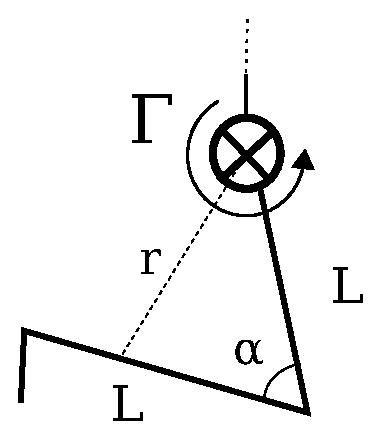
\includegraphics[width=0.12\textwidth]{leg_model.eps}
\end{figure}
慣性モーメントは次の形になる:

\begin{equation}
\begin{split}
\Gamma & \simeq \underbrace{\rho\int_0^L l^2 dl}_{太股} + \underbrace{\rho\int_0^L (L - l\cos\alpha)^2 + (l\sin\alpha)^2 dl}_{脛}\\
 & = \rho\left[l^3/3\right]_0^L + \rho\int_0^L (L^2 + l^2\cos^2\alpha - 2Ll\cos\alpha + l^2\sin^2\alpha) dl\\
 & = \rho L^3/3 + \int_0^L (L^2 + l^2 - 2Ll\cos\alpha) dl\\
 & = \rho L^3/3 + \rho\left(L^2\left[l\right]_0^L + \left[l^3/3\right]_0^L - 2L\cos\alpha\left[l^2/2\right]_0^L \right)\\
 & = \underbrace{\rho L^3/3}_{太股} + \underbrace{\rho L^3\left(4/3 - \cos\alpha  \right)}_{脛}
\end{split}
\end{equation}

慣性モーメントが低ければ低いほど足を前の方へ回すのに必要な力(トルク$\tau$)が少ない.\\
足を角度$\Delta\theta$回すのに必要なパワーは $W=\int_{\Delta\theta}\tau d\theta$ であるから、慣性モーメントが低ければ低いほど少ないパワーで足を回すことができる.
一定の歩幅(より正確には「一定の太股の振り幅」)で一定のスピードで走るときの消費エネルギーがその分減ることになる.
\\

その他考察:
\begin{itemize}
\item 慣性モーメントは重さに直接比例する:$\Gamma\propto\alpha$
\item 慣性モーメントは足の長さの3乗(!)に比例する:$\Gamma\propto{}L^3$
\end{itemize}

\newpage

以下は$\Gamma'=\Gamma/\rho{}L^3$の正規化された慣性モーメントのグラフと、トップレベル選手のフォームのときの値とホビーランナーのフォームのときを値を示し比較する.\\
トップアスリートのフォームはホビーランナーのフォームに比べて約50\%(以上)効率が良い結果になっている.\\
{\tiny{ ※注意 あくまで膝の曲げ角と消費エネルギーの関係についての結果のみになっている.全体的な効率の比較をするのに数多くのパラメータを考慮に入れる必要がある.}}

\begin{figure}[h!]
\centering
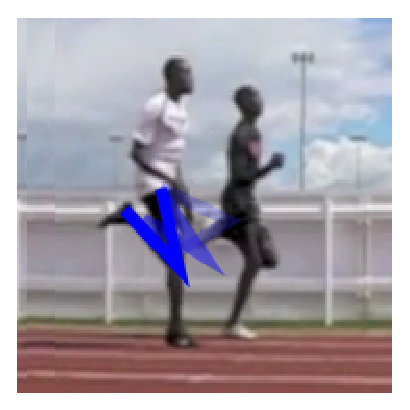
\includegraphics[width=0.15\textwidth]{img/kenyan_form.eps}
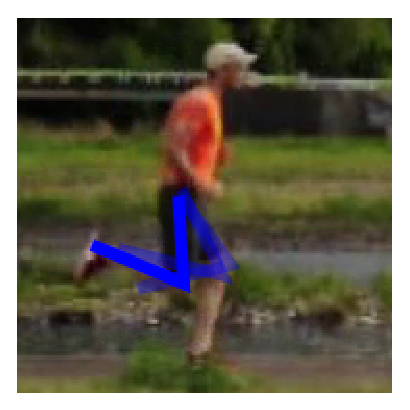
\includegraphics[width=0.15\textwidth]{img/form.eps} \\
\includegraphics[width=0.6\textwidth]{plot.eps}
\end{figure}


\raggedleft 以上

\end{document}